\appendix

%==========================================================================
\section{Notation}
\label{app:notation}

\Cref{tab:app-notation} collects the symbols used throughout.

\begin{table}[h]
\centering\small\setlength{\tabcolsep}{4pt}
\begin{tabular}{@{}ll@{}}
\toprule
Symbol & Meaning\\
\midrule
$Q$ & a zero-cost proxy (scalar per architecture)\\
$\acc$ & trained test accuracy (from the benchmark)\\
$T$ & early-training descent rate ($T_{\mathrm{slope}}$)\\
$\erank$ & effective rank of the at-init feature spectrum\\
$\params$ & parameter count\\
$\mathrm{cap}$ & capacity controls $\{\erank,\params\}$\\
$\rho,\ \corr$ & Spearman rank correlation (empirical)\\
$\Corr$ & Pearson correlation (Prop.~\ref{thm:bound})\\
$\partialcorr(\cdot,\cdot\mid\cdot)$ & rank partial correlation\\
$R^2_{\mathrm{res}}$ & out-of-fold $R^2$ on the capacity residual\\
$\Phimc$ & sub-$\sigma$-algebra of at-init (label-free) info\\
$S$ & a $\Phimc$-measurable (label-free) statistic\\
$Y$ & frozen at-init NTK kernel-regression error\\
$R^2_{\mathrm{cap}}$ & frozen-kernel resol.\ limit\\
$\mathrm{PC1}$ & leading principal component of the oriented zoo\\
$R_\alpha$ & R\'enyi-$\alpha$ effective rank ($\alpha{=}1$: NEAR)\\
\bottomrule
\end{tabular}
\caption{Notation.}
\label{tab:app-notation}
\end{table}

%==========================================================================
\section{Per-Conclusion Dependency Map}
\label{app:map}

The body states results top-down; this table maps each load-bearing conclusion
to its body location, key exhibit, and supporting appendix section.

\begin{table}[h]
\centering\small\setlength{\tabcolsep}{3pt}
\resizebox{\columnwidth}{!}{%
\begin{tabular}{@{}llll@{}}
\toprule
Conclusion & Body & Key fig./tab. & App.\ evidence\\
\midrule
Frozen-NTK bound & \cref{sec:theory} & \cref{eq:bound} & \cref{app:proof,app:ntk}\\
Capacity factor & \cref{sec:result1} & \cref{fig:results}a & \cref{app:pca-values}\\
Early-$T$ association & \cref{sec:result2} & \cref{tab:decomp-body} & \cref{app:replication}\\
At-init predictability & \cref{sec:result3} & \cref{fig:partials} & \cref{app:access-evidence}\\
No empirical ceiling & \cref{sec:result5} & \cref{fig:results}c & \cref{app:ntk}\\
Raw sign reversals & \cref{sec:result4} & \cref{fig:signflip} & \cref{app:perproxy-signflip}\\
Dimension sensitivity & \cref{sec:mechanism} & \cref{tab:app-spectral} & \cref{app:mechanism-evidence}\\
Broader portability & \cref{sec:generalize} & \cref{fig:portability} & \cref{app:generalize-evidence,app:replication}\\
Search trap costs & \cref{sec:searchtransfer} & \cref{tab:searchtransfer} & \cref{app:r2-search}\\
\bottomrule
\end{tabular}
}
\caption{\textbf{Per-conclusion dependency map.} Each load-bearing conclusion,
its body location, its key exhibit, and the appendix section carrying its full
evidence.}
\label{tab:app-map}
\end{table}

%==========================================================================
\section{The Proxy Zoo, Target $T$, and Sign Orientation}
\label{app:background}

This section fixes the three objects the body leans on but does not re-derive:
what a zero-cost proxy is, the kernel picture that \emph{motivates} (but does
not constrain) the decomposition, and the external trainability target $T$; it
then records the per-axis sign-orientation rule that every aggregate analysis
applies.

\paragraph{Zero-cost proxies.}
A zero-cost proxy scores an untrained network from a single
forward/backward pass and is used to rank candidates during search without
training~\cite{abdelfattah2021zerocost}. The thirteen standard proxies we
use are those collected in
NAS-Bench-Suite-Zero~\cite{krishnakumar2022nbsz}; our spectral arm
(\px{cond-sum}, \px{stable-sum}, $R_\alpha$) reimplements the
Dextr~\cite{dextr2025} and NEAR~\cite{near2025} functionals, parity-checked
in \cref{app:faithfulness}.

\paragraph{The kernel spectral-bias picture.}
For kernel regression / infinitely wide networks, the generalization error
decomposes over the kernel's Mercer spectrum
$\{\rho_i\}$ and the target coefficients $\{\bar c_i\}$
(\cref{app:external}). It cleanly separates a label-free \emph{capacity}
factor (the spectrum) from a label-dependent \emph{alignment} factor (the
coefficients), and motivates, without quantitatively constraining, our
decomposition. We import only this qualitative split; the lazy/NTK regime it
assumes need not hold at NB201 scale, consistent with an observed
capacity-orthogonal association with early training (\cref{sec:result2}).

\paragraph{The trainability target $T$.}
$T$ is the early-training learning rate read off the \emph{real} NATS-Bench
training curves ($\mathrm{hp}{=}12$, epochs $0$--$4$): the ordinary-least-squares
slope of the first five train-accuracy points (larger $T$ = faster early
learning). It is an external measurement (training curves, not proxies), so
partialling a proxy against $T$ compares against an outside quantity rather than
performing a self-consistency check.

\paragraph{Sign orientation (per axis).}
Proxies disagree on which direction predicts higher accuracy, so before any
aggregate analysis (the PCA of \cref{sec:r1}, the partials of \cref{sec:result3})
each proxy is oriented \emph{within each axis} by the sign of its Spearman
correlation with accuracy, falling back to the documented prior direction only
when the data correlation is negligible (\px{plain}, $\rho{=}{-}0.01$ on TSS;
\cref{sec:setup-orient}). This orientation is not bookkeeping: the sign a proxy
must be flipped on one axis can differ from the other. The corresponding raw
proxy--accuracy relationship is evaluated without orientation in
\cref{sec:result4}; the oriented residual direction is treated only as
sensitivity evidence. The full $29$-proxy zoo, its four groups, and the prior
directions are listed in \cref{tab:setup-zoo}.

%==========================================================================
\section{The Kernel Spectral-Bias Map, Restated}
\label{app:external}

We restate, for completeness, the kernel spectral-bias decomposition we use
qualitatively in \cref{sec:theory-map}. Following
Canatar et al.~\cite{canatar2021spectral} and Bordelon et
al.~\cite{bordelon2020spectrum}: for a kernel $K$ with Mercer eigenvalues
$\rho_1\ge\rho_2\ge\cdots$ and eigenfunctions $\{\phi_i\}$, and a target
$f^\star=\sum_i\bar c_i\phi_i$, the expected generalization error of kernel
ridge regression on $n$ samples takes the modal form
\begin{equation}
\label{eq:app-specbias}
\mathcal{E}(n)=\sum_i \bar c_i^{\,2}\,\mathcal{R}_i(n;\rho_1,\rho_2,\dots),
\end{equation}
where each modal factor $\mathcal{R}_i$ depends on the \emph{whole} spectrum
and decreases as mode $i$ becomes learnable. The split that matters for us:
$\{\rho_i\}$ is label-free (\emph{capacity}); $\{\bar c_i^{\,2}\}$ requires
the labels (\emph{alignment}). \emph{Used in:} \cref{sec:theory-map} to name
the two axes; no quantitative content is imported.

%==========================================================================
\section{Extended Related Work}
\label{app:related-ext}

The body \cref{sec:related} compresses five themes into one paragraph each; we
expand them here, reusing the same references. The unifying gap is that the
literature builds proxies that rank but rarely tests which observable factors
their scores track or whether those associations are stable across search spaces.

\paragraph{Capacity and expressivity proxies.}
A first line scores the richness an untrained network can express. NEAR's
effective rank~\cite{near2025} and the Dextr spectral condition
number~\cite{dextr2025} (whose \px{cond-sum} we reimplement at parity) summarize
the at-init feature spectrum, and Zen-NAS~\cite{lin2021zen} scores the response to
Gaussian perturbation. These are read as expressivity scores, but none asks how
much of every \emph{other} proxy is the same capacity number under another name;
\cref{sec:result1} shows a single component aligns strongly with effective rank
and carries about half the variance of the zoo.

\paragraph{Trainability and gradient proxies.}
A second line scores how easily a net will train from one-minibatch
gradient, Jacobian, or NTK statistics: ZiCo~\cite{li2023zico},
TE-NAS~\cite{chen2021tenas}, \px{jacob-cov}~\cite{jacobcov},
GradSign~\cite{gradsign}, and MeCo~\cite{jiang2023meco}. What is left open is
whether, with capacity held fixed, anything remains at init for them to read.
\cref{sec:result2,sec:result3} operationalizes this as the second term of the
decomposition: a capacity-orthogonal association with early training that is
partly predictable from label-free at-init statistics.

\paragraph{Ensembles and joint proxies.}
A third line mixes capacity and trainability into one recipe (AZ-NAS ensembles
four axes~\cite{aznas2024}, InTrain multiplies a capacity term by a
gradient-health term~\cite{intrain2026}, and SWAP-NAS scores sample-wise
activation patterns~\cite{peng2024swap}) on the implicit assumption that a single
combination transports across spaces. Several raw constituents reverse under
transport (\cref{sec:result4}), while SWAP and AZ-NAS remain positive on both
tested axes (\cref{app:r2-recent}). Recombination therefore requires explicit
transport validation rather than a universal sign assumption.

\paragraph{Benchmarks and the cross-space critique.}
A fourth line records the symptoms without a single account: rankings are
inconsistent across spaces and many proxies correlate with accuracy largely
through parameter count~\cite{ning2021evaluating,white2021powerful}, simple
hand-built features rival learned proxies~\cite{kadlecova2024graf}, and
NAS-Bench-Suite-Zero reports that combining $13$ proxies adds up to $+42\%$ over
the best single one~\cite{krishnakumar2022nbsz}. Our decomposition organizes these
symptoms into testable associations: ``proxies $\approx$ params'' corresponds to
the capacity-associated factor (\cref{sec:result1}), part of the remaining
complementarity is associated with the early-training target
(\cref{sec:result3}), and cross-space inconsistency appears as the sign reversals
of \cref{sec:result4}.

\paragraph{Kernel spectral bias.}
A fifth line, which we borrow only as a map, reads a label-free statistic's
reachable target through the kernel spectral-bias picture of
Canatar \etal~\cite{canatar2021spectral} and Bordelon \etal~\cite{bordelon2020spectrum}:
the at-init NTK's kernel-regression error. Our one formal statement
(\cref{thm:bound}) bounds that \emph{frozen} target, never trained accuracy. Some
proxies retain association with early training after the measured capacity controls
(\cref{sec:result2,sec:result3}). The proposition is motivation; the contribution is
the empirical analysis. The
body \cref{sec:related} is the compressed version.

%==========================================================================
\section{Proof of Proposition~\ref{thm:bound}}
\label{app:proof}

The body states the bound and defers the derivation here so the two copies
cannot drift. The argument is short, a conditional-expectation projection
followed by Cauchy--Schwarz, and the attainment case is recorded so the
``resolution limit'' reading is exact rather than loose.

\begin{proof}
By $0<\Var(Y)<\infty$ we have $\E[Y^2]<\infty$, so $\E[Y\mid\Phimc]$ exists in
$L^2$ and all covariances below are finite; $0<\Var(S)<\infty$ justifies the
final division.
Decompose $Y=\E[Y\mid\Phimc]+\varepsilon$ with
$\varepsilon:=Y-\E[Y\mid\Phimc]$. By linearity and idempotence of conditional
expectation $\E[\varepsilon\mid\Phimc]=0$, so for any $\Phimc$-measurable $S$,
\[
\operatorname{Cov}(S,\varepsilon)
=\E[S\,\varepsilon]-\E[S]\E[\varepsilon]
=\E\!\big[S\,\E[\varepsilon\mid\Phimc]\big]-0=0 .
\]
Hence $\operatorname{Cov}(S,Y)=\operatorname{Cov}\!\big(S,\E[Y\mid\Phimc]\big)$,
and by Cauchy--Schwarz
\[
\operatorname{Cov}(S,Y)^2
=\operatorname{Cov}\!\big(S,\E[Y\mid\Phimc]\big)^2
\le \Var(S)\,\Var\!\big(\E[Y\mid\Phimc]\big).
\]
Dividing by $\Var(S)\Var(Y)>0$,
\[
\Corr^2(S,Y)
=\frac{\operatorname{Cov}(S,Y)^2}{\Var(S)\Var(Y)}
\le \frac{\Var\!\big(\E[Y\mid\Phimc]\big)}{\Var(Y)}
= R^2_{\mathrm{cap}} .
\]
That $R^2_{\mathrm{cap}}\in[0,1]$ is immediate from the law of total variance,
$\Var(Y)=\Var\!\big(\E[Y\mid\Phimc]\big)+\E\!\big[\Var(Y\mid\Phimc)\big]\ge
\Var\!\big(\E[Y\mid\Phimc]\big)\ge 0$.
When $R^2_{\mathrm{cap}}>0$, taking $S=\E[Y\mid\Phimc]$ makes the
Cauchy--Schwarz step an equality, and $\Corr^2$ is invariant under affine
transformations of $S$, so the bound is attained; when $R^2_{\mathrm{cap}}=0$,
$\E[Y\mid\Phimc]$ is constant and the bound holds trivially for every admissible
$S$ (with $0<\Var(S)<\infty$).
\end{proof}

\noindent\textbf{Remark (scope).}
The bound holds for \emph{any} target $Y$; its content depends entirely on
which $Y$ one applies it to. We certify it only for $Y=$ the frozen at-init
NTK kernel-regression error. It does \emph{not} bound trained accuracy, and
\Cref{find:noceiling} shows the tempting ``ceiling'' reading does not
bind on NB201.

%==========================================================================
\section{Extended Results}
\label{app:extended}

This appendix collects the per-proxy numbers and sensitivity evidence
relocated from \cref{sec:cap-train,sec:crossspace} for length, together with
the longer positioning discussion. The results and the headline portability
heatmap (\cref{fig:portability}) remain in the body; the partial-slot heatmap
(\cref{fig:partials}, below) and the supporting per-proxy enumerations live here.

% Auto-generated supporting tables (per-proxy, PCA, portability, decomposition,
% setup) -- placed at the start of the Extended-results section so the six
% floats distribute through its prose rather than piling up (and stranding on a
% near-empty page) at the end of the appendix.
% HAND-FINALIZED appendix tables. Originally generated by
% theory/code/make_appendix_tables.py from zoo_analysis_out.txt + crossspace_out.txt,
% then hand-edited: proxy names de-coded to \px{...}, [htbp] floats, the NB201
% nwot/l2-norm/epe-nas portability cells filled, and the tab:setup-n / tab:setup-zoo
% tables added. THIS .tex IS THE SOURCE OF TRUTH. The generator is kept ONLY for
% number-provenance (every number still traces to a log); do NOT rerun it over this
% file -- a rerun would revert the hand edits and drop the two setup tables.

% ==== PERPROXY ====
\begin{table*}[htbp]\centering\small\setlength{\tabcolsep}{4pt}
\begin{tabular}{l rr r @{\hskip 1.5em} rr r}
\toprule
& \multicolumn{3}{c}{\textbf{TSS} ($n{=}324$)} & \multicolumn{3}{c}{\textbf{SSS} ($n{=}138$)}\\
\cmidrule(lr){2-4}\cmidrule(lr){5-7}
Proxy & $\rho(Q,\acc)$ & $\partialcorr(Q,T\!\mid\!\mathrm{cap})$ & $\rho(Q,\erank)$ & $\rho(Q,\acc)$ & $\partialcorr(Q,T\!\mid\!\mathrm{cap})$ & $\rho(Q,\erank)$\\
\midrule
\px{fisher} & $+0.47$ & $-0.152$ {\scriptsize$[-0.27,-0.04]$} & $+0.513$ & $+0.70$ & $+0.098$ {\scriptsize$[-0.09,+0.25]$} & $+0.728$\\
\px{grad-norm} & $+0.64$ & $-0.358$ {\scriptsize$[-0.44,-0.26]$} & $+0.747$ & $+0.59$ & $+0.074$ {\scriptsize$[-0.11,+0.24]$} & $+0.648$\\
\px{grasp} & $+0.55$ & $-0.176$ {\scriptsize$[-0.30,-0.04]$} & $+0.631$ & $-0.19$ & $-0.030$ {\scriptsize$[-0.19,+0.14]$} & $+0.198$\\
\px{snip} & $+0.64$ & $-0.369$ {\scriptsize$[-0.44,-0.28]$} & $+0.752$ & $+0.86$ & $+0.296$ {\scriptsize$[+0.11,+0.45]$} & $+0.899$\\
\px{synflow} & $+0.73$ & $-0.126$ {\scriptsize$[-0.22,-0.02]$} & $+0.781$ & $+0.94$ & $+0.332$ {\scriptsize$[+0.14,+0.48]$} & $+0.972$\\
\px{jacob-cov} & $+0.76$ & $+0.604$ {\scriptsize$[+0.52,+0.67]$} & $+0.726$ & $-0.00$ & $-0.124$ {\scriptsize$[-0.29,+0.06]$} & $+0.025$\\
\px{plain} & $-0.01$ & $-0.170$ {\scriptsize$[-0.28,-0.06]$} & $-0.013$ & $+0.06$ & $+0.131$ {\scriptsize$[-0.05,+0.29]$} & $+0.069$\\
\px{zico} & $+0.78$ & $-0.197$ {\scriptsize$[-0.29,-0.09]$} & $+0.880$ & $+0.86$ & $+0.233$ {\scriptsize$[+0.06,+0.40]$} & $+0.887$\\
\px{meco} & $+0.88$ & $+0.291$ {\scriptsize$[+0.17,+0.40]$} & $+0.856$ & $-0.79$ & $-0.398$ {\scriptsize$[-0.51,-0.23]$} & $+0.910$\\
\px{zen} & $-0.10$ & $-0.049$ {\scriptsize$[-0.15,+0.05]$} & $+0.146$ & $+0.90$ & $+0.517$ {\scriptsize$[+0.37,+0.63]$} & $+0.932$\\
\px{ntk} & $-0.78$ & $+0.180$ {\scriptsize$[+0.06,+0.30]$} & $+0.774$ & $-0.20$ & $+0.241$ {\scriptsize$[+0.07,+0.39]$} & $+0.139$\\
\px{gradsign} & $+0.78$ & $-0.135$ {\scriptsize$[-0.23,-0.03]$} & $+0.810$ & $+0.86$ & $-0.130$ {\scriptsize$[-0.29,+0.09]$} & $+0.937$\\
\px{cond-sum} & $+0.88$ & $+0.215$ {\scriptsize$[+0.09,+0.33]$} & $+0.893$ & $-0.77$ & $-0.141$ {\scriptsize$[-0.31,+0.04]$} & $+0.830$\\
\px{stable-sum} & $+0.86$ & $+0.109$ {\scriptsize$[-0.02,+0.23]$} & $+0.971$ & $+0.68$ & $-0.014$ {\scriptsize$[-0.17,+0.15]$} & $+0.740$\\
$R_{\alpha=0.5}$ & $+0.84$ & $-0.266$ {\scriptsize$[-0.36,-0.13]$} & $+0.993$ & $+0.90$ & $-0.295$ {\scriptsize$[-0.44,-0.03]$} & $+0.997$\\
$R_{\alpha=2}$ & $+0.88$ & $+0.256$ {\scriptsize$[+0.12,+0.37]$} & $+0.995$ & $+0.91$ & $+0.067$ {\scriptsize$[-0.13,+0.26]$} & $+0.995$\\
$R_{\alpha=4}$ & $+0.88$ & $+0.245$ {\scriptsize$[+0.12,+0.35]$} & $+0.989$ & $+0.89$ & $-0.010$ {\scriptsize$[-0.19,+0.17]$} & $+0.976$\\
$R_{\alpha=8}$ & $+0.88$ & $+0.223$ {\scriptsize$[+0.09,+0.34]$} & $+0.985$ & $+0.88$ & $+0.006$ {\scriptsize$[-0.14,+0.18]$} & $+0.959$\\
$R_{\alpha=16}$ & $+0.87$ & $+0.205$ {\scriptsize$[+0.08,+0.31]$} & $+0.984$ & $+0.87$ & $+0.015$ {\scriptsize$[-0.15,+0.19]$} & $+0.946$\\
\px{Q-ntk-logcond} & $+0.30$ & $-0.121$ {\scriptsize$[-0.24,+0.01]$} & $+0.405$ & $-0.53$ & $-0.475$ {\scriptsize$[-0.62,-0.30]$} & $+0.659$\\
\px{Q-ntk-logtrace} & $-0.36$ & $-0.075$ {\scriptsize$[-0.18,+0.03]$} & $+0.404$ & $+0.29$ & $-0.032$ {\scriptsize$[-0.21,+0.14]$} & $+0.292$\\
\px{Q-ntk-effrank} & $-0.50$ & $+0.105$ {\scriptsize$[+0.00,+0.21]$} & $+0.565$ & $+0.58$ & $-0.343$ {\scriptsize$[-0.52,-0.14]$} & $+0.667$\\
\px{Q-ntk-loglmax} & $-0.36$ & $-0.078$ {\scriptsize$[-0.18,+0.04]$} & $+0.406$ & $-0.11$ & $-0.198$ {\scriptsize$[-0.32,-0.06]$} & $+0.196$\\
\px{Q-zico-rand} & $+0.31$ & $+0.207$ {\scriptsize$[+0.08,+0.32]$} & $+0.310$ & $+0.09$ & $+0.121$ {\scriptsize$[-0.06,+0.29]$} & $+0.120$\\
\px{Q-zico-rot} & $+0.40$ & $+0.183$ {\scriptsize$[+0.06,+0.30]$} & $+0.392$ & $+0.07$ & $-0.045$ {\scriptsize$[-0.20,+0.14]$} & $+0.077$\\
\px{Q-coh-rand} & $-0.48$ & $-0.072$ {\scriptsize$[-0.16,+0.03]$} & $+0.535$ & $-0.09$ & $+0.075$ {\scriptsize$[-0.13,+0.26]$} & $+0.133$\\
\px{Q-coh-rot} & $+0.08$ & $+0.128$ {\scriptsize$[+0.04,+0.21]$} & $+0.038$ & $-0.24$ & $-0.205$ {\scriptsize$[-0.38,-0.01]$} & $+0.282$\\
\px{Q-adapt-rot} & $+0.10$ & $+0.143$ {\scriptsize$[+0.03,+0.24]$} & $+0.041$ & $+0.65$ & $-0.602$ {\scriptsize$[-0.70,-0.47]$} & $+0.809$\\
\px{Q-zico-oracle}$^{\mathrm{L}}$ & $+0.35$ & $+0.253$ {\scriptsize$[+0.13,+0.37]$} & $+0.334$ & $+0.05$ & $+0.040$ {\scriptsize$[-0.13,+0.22]$} & $+0.060$\\
\bottomrule\end{tabular}
\caption{\textbf{Complete per-proxy NB201 results (full-zoo)} on the topology
(TSS) and size (SSS) axes; the partial columns are rendered as body
\cref{fig:partials}. $\rho(Q,\acc)$ is shown raw and $^{\mathrm{L}}$\,\px{Q-zico-oracle}
uses labels (excluded from all label-free claims).}
\label{tab:app-perproxy}
\end{table*}

% ==== PCA ====
\begin{table}[htbp]\centering\small\setlength{\tabcolsep}{4pt}
\begin{tabular}{lr @{\hskip 1.2em} lr}
\toprule
\multicolumn{2}{c}{\textbf{TSS} (PC1, 52.9\% var)} & \multicolumn{2}{c}{\textbf{SSS} (PC1, 49.4\% var)}\\
\cmidrule(lr){1-2}\cmidrule(lr){3-4}
Proxy & loading & Proxy & loading\\\midrule
$R_{\alpha=16}$ & $+0.246$ & $R_{\alpha=0.5}$ & $+0.260$\\
$R_{\alpha=8}$ & $+0.246$ & $R_{\alpha=2}$ & $+0.260$\\
$R_{\alpha=4}$ & $+0.246$ & \px{synflow} & $+0.257$\\
\px{stable-sum} & $+0.245$ & $R_{\alpha=4}$ & $+0.256$\\
$R_{\alpha=2}$ & $+0.244$ & $R_{\alpha=8}$ & $+0.253$\\
$R_{\alpha=0.5}$ & $+0.233$ & $R_{\alpha=16}$ & $+0.250$\\
\px{cond-sum} & $+0.231$ & \px{gradsign} & $+0.247$\\
\px{snip} & $+0.225$ & \px{meco} & $+0.245$\\
\px{grad-norm} & $+0.225$ & \px{zen} & $+0.244$\\
\px{ntk} & $+0.224$ & \px{snip} & $+0.240$\\
\px{meco} & $+0.215$ & \px{zico} & $+0.235$\\
\px{zico} & $+0.211$ & \px{Q-adapt-rot} & $+0.227$\\
\px{gradsign} & $+0.201$ & \px{cond-sum} & $+0.225$\\
\px{jacob-cov} & $+0.194$ & \px{stable-sum} & $+0.200$\\
\bottomrule\end{tabular}
\caption{\textbf{Leading principal component of the oriented zoo (top-14 loadings;
$n{=}317/138$ complete cases),}
which loads broadly across the spectral and gradient proxies;
$\corr(\mathrm{PC1},\erank){=}{+}0.937$ (TSS) / ${+}0.986$ (SSS).}
\label{tab:app-pca}
\end{table}

% ==== PORTABILITY ====
\begin{table*}[htbp]\centering\small\setlength{\tabcolsep}{4pt}
\begin{tabular}{lrrrrrrr}
\toprule
Proxy & NB101 & NB201-c10 & NB201-c100 & NB201-IN16 & NB301 & TNAS-obj & TNAS-sc\\\midrule
\px{grad-norm} & $+0.509$ & $+0.595$ & $+0.640$ & $+0.580$ & $\mathbf{-0.153}$ & $+0.389$ & $+0.650$\\
\px{snip} & $+0.539$ & $+0.595$ & $+0.642$ & $+0.579$ & $\mathbf{-0.162}$ & $+0.431$ & $+0.684$\\
\px{fisher} & $+0.501$ & $+0.394$ & $+0.427$ & $+0.361$ & $\mathbf{-0.338}$ & $+0.464$ & $+0.655$\\
\px{jacob-cov} & $\mathbf{-0.526}$ & $+0.721$ & $+0.700$ & $+0.677$ & $\mathbf{-0.075}$ & $+0.604$ & $+0.783$\\
\px{synflow} & $+0.693$ & $+0.737$ & $+0.766$ & $+0.757$ & $+0.221$ & $+0.466$ & $+0.647$\\
\px{nwot} & $+0.323$ & $+0.755$ & $+0.800$ & $+0.775$ & $+0.565$ & $+0.320$ & $+0.517$\\
\px{zen} & $+0.651$ & $\mathbf{-0.065}$ & $\mathbf{-0.086}$ & $\mathbf{-0.017}$ & $+0.470$ & $+0.495$ & $+0.669$\\
\px{grasp} & $\mathbf{-0.102}$ & $+0.510$ & $+0.556$ & $+0.504$ & $+0.205$ & $\mathbf{-0.390}$ & $\mathbf{-0.566}$\\
\px{l2-norm} & $+0.547$ & $+0.678$ & $+0.719$ & $+0.703$ & $+0.461$ & $+0.268$ & $+0.495$\\
\px{plain} & $+0.047$ & $\mathbf{-0.082}$ & $\mathbf{-0.081}$ & $\mathbf{-0.053}$ & $\mathbf{-0.295}$ & $+0.516$ & $+0.326$\\
\px{params} & $+0.670$ & $+0.717$ & $+0.735$ & $+0.702$ & $+0.502$ & $+0.387$ & $+0.577$\\
\px{flops} & $+0.478$ & $+0.717$ & $+0.735$ & $+0.702$ & $+0.470$ & $\mathbf{-0.048}$ & $\mathbf{-0.125}$\\
\px{epe-nas} & $\mathbf{-0.080}$ & $+0.704$ & $+0.691$ & $+0.665$ & $\mathbf{-0.011}$ & $+0.520$ & $+0.432$\\
\bottomrule\end{tabular}
\caption{\textbf{Cross-benchmark portability matrix:} Spearman $\corr(Q,\acc)$
point estimates for each standard proxy (\textbf{bold}${=}$negative), rendered
as body \cref{fig:portability}. Sample
sizes are NB101 $100$, NB301 $50$, and TransNAS $150$. NB201 is $1000$ except
\px{jacob-cov}, \px{zen}, and \px{epe-nas} ($977$) and \px{nwot} ($984$). Strict-case
intervals are in \cref{app:generalize-evidence}.}
\label{tab:app-portability}
\end{table*}

% ==== DECOMP ====
\begin{table}[htbp]\centering\small\setlength{\tabcolsep}{5pt}
\begin{tabular}{ll rr}
\toprule
Dataset & Features & $R^2_{\mathrm{in}}$ & $R^2_{\mathrm{cv}}$\\\midrule
CIFAR-10 & params & $0.526$ & $+0.526$\\
CIFAR-10 & params+T & $0.779$ & $+0.775$\\
CIFAR-10 & params+erank & $0.732$ & $+0.730$\\
CIFAR-10 & params+T+erank & $0.831$ & $+0.828$\\
\midrule
CIFAR-100 & params & $0.541$ & $+0.541$\\
CIFAR-100 & params+T & $0.748$ & $+0.743$\\
CIFAR-100 & params+erank & $0.780$ & $+0.778$\\
CIFAR-100 & params+T+erank & $0.843$ & $+0.840$\\
\midrule
IN16-120 & params & $0.480$ & $+0.482$\\
IN16-120 & params+T & $0.776$ & $+0.777$\\
IN16-120 & params+erank & $0.726$ & $+0.727$\\
IN16-120 & params+T+erank & $0.837$ & $+0.837$\\
\bottomrule\end{tabular}
\caption{\textbf{The capacity/trainability decomposition replicates across the
three NB201 datasets} ($n{=}324$; rank-$R^2$ of accuracy, in-sample and
leakage-clean 5-fold CV); the $R^2_{\mathrm{cv}}$ slice is body
\cref{tab:decomp-body}. This arm uses curve-derived accuracy and the
train-accuracy $T$ (\cref{sec:app-xspace-method}).}
\label{tab:app-decomp}
\end{table}

% ==== SETUP-N (relocated from sec/3_setup.tex) ====
\begin{table}[htbp]
  \centering
  \small
  \begin{tabular}{lcc}
    \toprule
    Population & TSS & SSS \\
    \midrule
    Full-zoo table intersection (before finite mask) & 324 & 138 \\
    PCA-complete 29-feature population      & 317 & 138 \\
    Standard-proxy base table              & 1000 & 425 \\
    \quad of which erank / $T$ present      & 324 & 138 \\
    \bottomrule
  \end{tabular}
  \caption{Sample sizes per search-space axis. The full-zoo join precedes
  analysis-specific finite-value masks; the fixed PCA mask leaves $317/138$
  complete cases. The standard-proxy population covers more architectures but
  fewer proxies. The SSS arm ($n{=}138$) is the binding sample-size constraint.}
  \label{tab:setup-n}
\end{table}

% ==== SETUP-ZOO (relocated from sec/3_setup.tex) ====
\begin{table}[htbp]
  \centering
  \small
  \setlength{\tabcolsep}{3pt}
  \begin{tabular}{p{0.26\linewidth}p{0.07\linewidth}p{0.52\linewidth}}
    \toprule
    Group & \# & Members \\
    \midrule
    Standard & 12 &
      \px{fisher, grad-norm, grasp, snip, synflow, jacob-cov, plain, zico, meco,
      zen, ntk, gradsign} \\
    Spectral & 7 &
      \px{cond-sum, stable-sum}, $R_{\alpha=0.5,2,4,8,16}$ \\
    Label-free probes & 9 &
      \px{Q-ntk-\{logcond, logtrace, effrank, loglmax\}, Q-zico-\{rand, rot\},
      Q-coh-\{rand, rot\}, Q-adapt-rot} \\
    Label oracle (flagged) & 1 & \px{Q-zico-oracle} \\
    \midrule
    \textbf{Total} & \textbf{29} & \\
    \bottomrule
  \end{tabular}
  \caption{The 29-feature aligned zoo. $R_{\alpha=1}$ is held out as the
  effective-rank capacity anchor. Per-axis outcome orientation is accompanied by
  raw and globally fixed controls
  (\cref{sec:setup-orient}). The single label-using oracle is held apart as an
  upper reference.}
  \label{tab:setup-zoo}
\end{table}



\begin{figure*}[t]
  \centering
  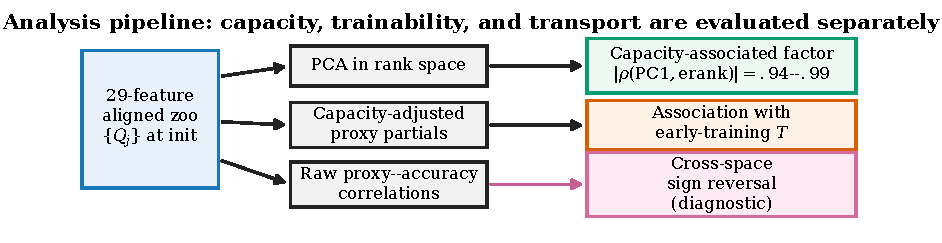
\includegraphics[width=\textwidth]{figures/fig2_overview.pdf}
  \caption{\textbf{Analysis pipeline.} A 29-feature aligned zoo is summarized
  by a capacity-associated factor (PC1 scores track effective rank) and a
  capacity-orthogonal trainability residual. Raw proxy/accuracy reversals are
  orientation-free; per-proxy residual directions use the stated orientation
  rule and are treated as sensitivity evidence. Proposition~\ref{thm:bound}
  concerns only the frozen at-init NTK target $Y$.}
  \label{fig:overview}
\end{figure*}

\subsection{Per-proxy values for the sign-flip}
\label{app:perproxy-signflip}

The headline (\cref{find:flip}) is that the \emph{same} raw proxy reverses sign
across the two axes. We report the orientation-free accuracy correlation
(\emph{accuracy slot}) and, separately, the capacity-residual trainability
partial under per-axis outcome-informed orientation. The latter is an
orientation-sensitive secondary analysis, not independent evidence for the raw
flip.

\paragraph{Accuracy slot.}
The NB201 columns of \cref{fig:portability} (full numbers in
\cref{tab:app-perproxy}) give $\corr(Q,\acc)$ for the proxies whose
orientation is not preserved across axes. Our inverse-condition-sum
spectral functional moves from $\corr(Q,\acc)=+0.88$ on TSS to $-0.77$ on
SSS; \px{meco} from $+0.88$ to $-0.79$; \px{grasp} from $+0.55$ to
$-0.19$ (\cref{fig:signflip}). These are not weak proxies noisy near zero:
\px{cond-sum} and \px{meco} are among the strongest single proxies on TSS and
among the most strongly \emph{anti}-correlated on SSS, so a practitioner who
calibrated on topology would, on size, be selecting \emph{against} accuracy.

\begin{figure}[t]
  \centering
  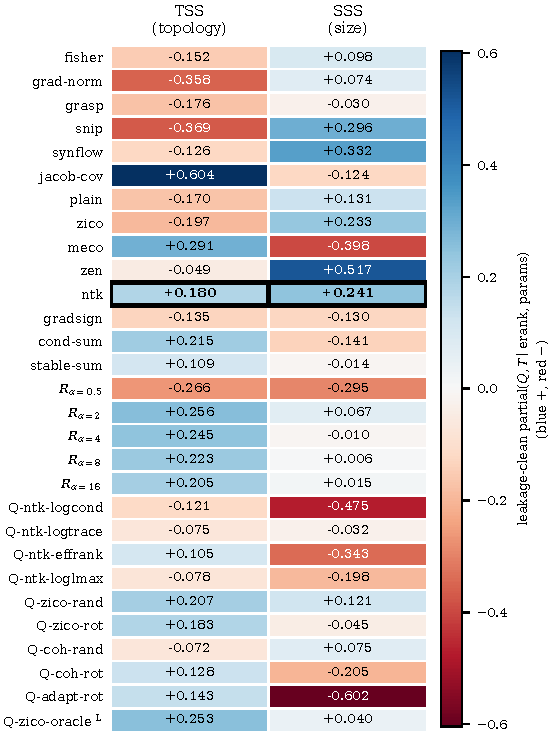
\includegraphics[width=\columnwidth]{figures/fig5_partials.pdf}
  \caption{\textbf{Outcome-oriented trainability partials.} Leakage-clean
  partial $\partialcorr(Q,T\mid\erank,\params)$ for every proxy on TSS ($x$)
  versus SSS ($y$), after outcome-informed per-axis orientation. The global
  orientation control shows that directional quadrant membership is sensitive
  to this rule (\cref{app:r2-orientation}).}
  \label{fig:partials}
\end{figure}

\paragraph{Trainability slot under outcome-informed orientation.}
\Cref{fig:partials} (full numbers in \cref{tab:app-perproxy}) reports the leakage-clean partial
correlation $\partialcorr(Q,T\mid\erank,\params)$, the trainability
signal a proxy accesses after capacity is regressed out
(\cref{sec:result3}). \px{jacob-cov}, the single best label-free
route to trainability on TSS ($\partialcorr=+0.604$ $[+0.52,+0.67]$),
collapses to $-0.124$ $[-0.29,+0.06]$ on SSS: its access does not merely
weaken, it disappears and turns mildly negative. \px{meco} flips from
$+0.291$ $[+0.17,+0.40]$ to $-0.398$ $[-0.51,-0.23]$; \px{cond-sum}
from $+0.215$ $[+0.09,+0.33]$ to $-0.141$ $[-0.31,+0.04]$. Our label-free
adaptation probe \px{Q-adapt-rot} shows the most extreme reversal,
from $+0.143$ $[+0.03,+0.24]$ on TSS to $-0.602$ $[-0.70,-0.47]$ on SSS;
\px{gradsign} changes from a (standard-arm) $+0.11$ to $-0.130$
$[-0.29,+0.09]$. Because the orientation itself uses accuracy separately on
each axis, these signs are not independent evidence of transport; the raw
accuracy-slot reversals remain the orientation-free result.

\paragraph{Narrow survivor under outcome-informed orientation.}
Applying the conservative two-sided test from \cref{sec:result3} under this
rule, the only full-zoo proxy that passes is \px{ntk}, in the
\emph{trainability partial} slot $\partialcorr(Q,T\mid\erank,\params)$ (not
the raw-correlation slot): $+0.180$
$[+0.06,+0.30]$ TSS; $+0.241$ $[+0.07,+0.39]$ SSS. At the larger base
sample of the standard-proxy arm two more clear the bar, \px{synflow}
and \px{zico}, giving $\{$\px{synflow}, \px{zico},
\px{ntk}$\}$. Under that rule, few topology-axis carriers retain the same sign
on the size axis (\cref{fig:results}b). Under the globally fixed rule, both
\px{meco} and \px{ntk} have positive marginal intervals on both axes; this
comparison is exploratory and unadjusted, so no orientation-robust uniqueness
claim is made.

\subsection{Dimension-linked sensitivity evidence}
\label{app:mechanism-evidence}

Having shown the raw flip, we test whether representation geometry accompanies
it. This account is observational: several scores depend numerically on spectral
dimension, and the two axes vary topology and width differently. The controls
below support a dimension-linked interpretation but do not identify a mechanism.

\paragraph{Observed axis dependence.}
Several reversing scores are functionals of the representation spectrum
(condition number, feature covariance, or Jacobian/NTK quantities) whose
numerical value depends on representation geometry. TSS holds width fixed while
varying topology; SSS varies width directly. This makes dimension-linked score
behavior plausible, but the observational comparison cannot determine which
architectural quantity causes the reversal.

\paragraph{Scope of the SSS-side association.}
On the SSS (size/width) axis, effective-rank conditioning greatly weakens the
observed association, suggesting a dimension/capacity-linked component rather
than an independent mechanism. This is not a mediation test or a validated
representation-dimension match: the available cached count is not a validated
dimension field, and its support does not overlap across axes
(\cref{app:r2-dimension}). The \px{cond-sum} SSS raw correlation
$\corr(Q,\acc)$ is $-0.768$; it
collapses when we condition on effective rank ($-0.047$, $95\%$CI
$[-0.242,+0.128]$, spanning zero) and on params${+}$erank jointly ($-0.048$,
$[-0.260,+0.130]$), while conditioning on \emph{params alone} leaves it
intact ($-0.317$, $[-0.478,-0.128]$). The \px{meco}/\px{jacob-cov}/\px{grasp}
SSS partials collapse under the same effective-rank control. The TSS-side
positive partials are \emph{not} explained away by capacity: \px{jacob-cov}
$+0.604$ and \px{cond-sum} $+0.215$ both survive BH-FDR and Holm correction.

\paragraph{The spectral family exposes the dependence.}
Within our own spectral family the descriptive dependence is visible
(\cref{sec:faithfulness}): the inverse-condition-sum \px{cond-sum}, a
pure conditioning functional, is exactly the one that flips ($+0.887$ TSS /
$-0.781$ SSS on the $n{=}500$ spectral-arm population; the full-zoo $n{=}324$
values used in the body and conclusion are the rounded $+0.88$ / $-0.77$),
whereas the R\'enyi effective-rank functionals $R_\alpha$,
which integrate over the whole spectrum rather than its conditioning, remain
positive on both axes (e.g.\ $R_{\alpha=1}$, NEAR's effective rank,
$+0.864$ / $+0.911$; $R_{\alpha=2}$, $+0.879$ / $+0.912$). The choice of
spectral summary is associated with whether a proxy ports across axes. Frozen
cross-space transfer also degrades asymmetrically: a linear model fit on TSS
assigns \px{cond-sum} a positive weight and reaches transfer Spearman $+0.5405$
on SSS, whereas a model fit on SSS down-weights the sign-unstable functional
and transfers back to TSS at $+0.8629$.

\subsection{Generalization across search spaces (per-space values)}
\label{app:generalize-evidence}

Sign reversals are also observed outside the two NB201 axes
(\cref{find:generalize}). This subsection lists the four strictly supported
instances, then reports multiplicity controls for the larger grid.

Under the bootstrap-CI quarantine ($2000$ resamples; CI-separated $=$ the two
spaces' $95\%$ intervals disjoint), four flips are load-bearing:
\px{jacob-cov} $+0.78\,[+0.69,+0.85]$ on TransNAS-scene vs.\
$-0.53\,[-0.67,-0.35]$ on NB101; \px{grasp} $+0.56\,[+0.51,+0.60]$ on
NB201-CIFAR-100 vs.\ $-0.57\,[-0.69,-0.43]$ on TransNAS-scene; \px{zen}
$+0.67\,[+0.55,+0.76]$ on TransNAS-scene vs.\ $-0.09\,[-0.16,-0.01]$ on
NB201-CIFAR-100; and \px{plain} $+0.33\,[+0.15,+0.47]$ on TransNAS-scene
vs.\ $-0.08\,[-0.14,-0.02]$ on NB201-CIFAR-10. For \px{jacob-cov} and
\px{grasp} both sides are large; for \px{zen} and \px{plain} the
negative side is mild but its CI excludes zero (large-$n$ NB201 arms).
With all $13$ proxies scored on the TransNAS-object column ($n{=}150$), these
four cases remain unchanged: \px{flops} and \px{epe-nas}
reverse only to near-zero on TransNAS (CIs spanning zero) and stay suggestive, and
only NB301 ($n{=}50$, disjoint $0/50$) remains excluded as degenerate. The full
$13\times7$ portability matrix with bootstrap intervals is in \cref{app:crossspace}.

\paragraph{Multiplicity control.}
The four strict instances remain supported under the reported multiplicity
controls. On the per-proxy early-training partial
grid ($58$ cells, $\partialcorr(Q,T_{\mathrm{slope}}\mid\erank,\params)$ over
$29$ proxies $\times$ two spaces, $5000$ Freedman--Lane permutations per cell),
$34$ cells survive BH-FDR at $\alpha{=}0.05$ ($25$ survive the conservative
Benjamini--Yekutieli, $23$ survive Holm--Bonferroni). On the portability grid
($91$ finite cells, including the full TransNAS-object
column), $78$ survive BH-FDR and $72$ survive Holm. Each of the four load-bearing
flips is itself FDR-significant (\cref{tab:app-fdr}); the apparent
\px{grad-norm}/\px{snip}/\px{fisher}/\px{epe-nas} candidate flips occur only in
small-$n{=}50$ NB301-CIFAR-10 attenuation cells ($|\rho|\le0.34$), and \px{flops}
reverses only to near-zero on TransNAS; none meets the strict support rule. The \px{ntk} $T_{\mathrm{slope}}$
partial survives BH-FDR in \emph{both} spaces (TSS $+0.180$, perm $p{=}0.0016$;
SSS $+0.241$, perm $p{=}0.0054$).

\begin{table}[t]
\centering\small\setlength{\tabcolsep}{4.5pt}
\begin{tabular}{llrrc}
\toprule
Proxy & Space & $\rho$ & perm $p$ & $n$\\
\midrule
\px{jacob-cov} & NB101-CIFAR-10  & $-0.526$ & $2.0{\times}10^{-4}$ & $100$\\
\px{grasp}     & TransNAS-scene  & $-0.566$ & $2.0{\times}10^{-4}$ & $150$\\
\px{zen}       & NB201-CIFAR-100 & $-0.086$ & $6.2{\times}10^{-3}$ & $977$\\
\px{plain}     & TransNAS-scene  & $+0.326$ & $2.0{\times}10^{-4}$ & $150$\\
\bottomrule
\end{tabular}
\caption{\textbf{Each load-bearing flip is FDR-significant} (the flip cell shown;
all four pass BH-FDR, three also Holm).}
\label{tab:app-fdr}
\end{table}

The capacity/trainability decomposition itself
replicates across the three NB201 datasets (\cref{app:crossspace},
\cref{tab:app-decomp}): parameters explain $R^2\approx0.48$--$0.54$, and
adding either the trainability target $T$ ($\sim{+}0.25$) or effective rank
($\sim{+}0.23$) lifts $R^2$ comparably; the joint model including both reaches
$\sim0.83$ (these are nested-model $R^2$ values, not additive terms of
\cref{eq:decomp}).

\subsection{Replication across the NB201 datasets}
\label{app:replication}

We apply the same analysis protocol
(\cref{sec:result1,sec:result2,sec:result3}) to NB201's three datasets.
\Cref{tab:app-replication} shows the descriptive pattern recurs: capacity is
the dominant baseline, adding ground-truth $T$ increases rank-$R^2$, and a
capacity-surviving complementarity gain persists. The capacity-anchored
trainability partial reproduces the headline value: with effective rank as the
capacity control ($n{=}324$),
$\partialcorr(T,\acc\mid\erank,\params){=}{+}0.608/{+}0.536/{+}0.635$ on
CIFAR-10/CIFAR-100/ImageNet16-120 (cf.\ ${+}0.602$ in the main analysis), and the
spectral PCA again aligns with effective rank
($\corr(\mathrm{PC1},\erank){=}{+}0.96$, PC1 $\sim\!69\%$ variance).

\begin{table}[t]
\centering\small\setlength{\tabcolsep}{3pt}
\begin{tabular}{l r rr r r}
\toprule
Benchmark / dataset & $n$ & \multicolumn{2}{c}{rank-$R^2(\acc)$} & $\Delta_T$ & res.\ gain\\
\cmidrule(lr){3-4}
 & & $|\,\mathrm{cap}$ & $+T$ & share & (cap-surv.)\\
\midrule
NB201 / CIFAR-10      & 1000 & $0.51$ & $0.79$ & $+0.28$ & $+33\%$\\
NB201 / CIFAR-100     & 1000 & $0.54$ & $0.75$ & $+0.21$ & $+44\%$\\
NB201 / IN16-120      & 1000 & $0.49$ & $0.78$ & $+0.29$ & $+49\%$\\
\bottomrule
\end{tabular}
\caption{\textbf{The descriptive capacity-plus-$T$ pattern recurs} across
NB201's three datasets (params-anchored, leakage-clean): the capacity baseline
explains $0.49$--$0.54$ of accuracy rank and ground-truth $T$ adds a positive
increment $\Delta_T$.}
\label{tab:app-replication}
\end{table}

\subsection{Empirically instantiating Proposition~\ref{thm:bound}: the NTK target}
\label{app:ntk}

The Proposition is a yardstick, not a headline, and this subsection earns that
status by measurement rather than assumption. We compute its target, show what
a label-free dictionary explains, report a negative result (even the frozen
kernel is not a pure-capacity object), and test whether this at-init target is a
useful surrogate for trained accuracy. It is not: the bound prices $Y$ exactly
and remains silent on accuracy, as scoped in the body.

\paragraph{Computing the target.}
Proposition~\ref{thm:bound}'s target $Y$ is usually only \emph{described}; here we
\emph{compute} it (at init). For each of the $324$ full-zoo
NB201-TSS architectures we form the weight-only empirical NTK Gram over a fixed
CIFAR-10 batch ($m{=}256$ samples with $m{<}P$, so the Gram is rank-$\le m$ and
KRR interpolates; $5$ batches) and take $Y$ as the held-out
kernel-ridge-regression MSE against the real labels (closed-form; the quantity
\cref{eq:app-specbias} describes). This is a weight-only at-init NTK at one
operating point, not the full NTK. $Y$ is rank-stable across batches
(Spearman$(\text{batch}_0,\text{batch}_4){=}0.85$).

\noindent\textbf{What a finite label-free dictionary explains.} On the
across-architecture ensemble the full $\sigma$-algebra contains the architecture
identity, so $Y$ is arch-determined and the proposition's $R^2_{\mathrm{cap}}{=}1$
exactly, vacuous (\cref{sec:theory-bound}, point~(iii)). The non-trivial object
is therefore the variance of $Y$ explained by a \emph{pre-declared finite
label-free dictionary} $F$ ($30$ features: NTK-Gram spectral summaries, our
spectral proxies, and the gradient/zoo proxies): $R^2(F\!\to\!Y){=}0.81$ (rank-CV
$R^2{=}0.8112$; the matching $L^2$ in-sample Pearson
estimate is $R^2{\approx}0.6645$). We do \emph{not} call this $R^2(F\!\to\!Y)$ a
``resolution limit'': it is one dictionary's explained variance, not the proposition's
$R^2_{\mathrm{cap}}$. On these data every single proxy's squared rank correlation with $Y$ stays below
the dictionary's rank-CV $R^2$ (max single $0.68$ vs.\ $0.81$); no proposition forces
this: it is an empirical observation, not a Pearson instance of
Proposition~\ref{thm:bound}.

\noindent\textbf{Even the frozen kernel is not a pure-capacity object.} Among
the proxies (excluding functions of $K_a$), the \emph{gradient} family
predicts $Y$ better than the \emph{spectral/capacity} family (best $0.68$ vs.\
$0.42$; family gap $-0.2591\,[-0.3367,-0.1862]$, CI-separated). The naive ``$Y$ is governed by
the spectrum'' reading is thus not supported even for the frozen-kernel target.
We report this as a negative result.

\noindent\textbf{Coherence: the at-init NTK target is a weak surrogate for trained accuracy.}
The same dictionary explains $Y$ ($0.81$) and trained accuracy (rank-CV
$R^2{=}0.89$) comparably, yet the per-architecture at-init NTK error $Y$
correlates only
$\rho{=}0.40\,[0.29,0.49]$ with trained accuracy (robust across the ridge:
$\rho{=}0.11/0.40/0.47$ for $\lambda_K{=}0.01/0.1/1$). These NB201-TSS
(CIFAR-10) observations do not support treating this frozen at-init NTK target as
a quantitative surrogate for trained accuracy: Proposition~\ref{thm:bound}
prices $Y$ exactly but is silent on accuracy, consistent with the narrow scope in
\cref{sec:theory} and \cref{find:noceiling}. The best
single proxy reaches $R^2{=}0.78$ against accuracy, \emph{not} bounded by
$R^2(F\!\to\!Y){=}0.81$: different targets, no proposition forcing the at-init ceiling
onto accuracy.

\subsection{PC1 correlations}
\label{app:pca-values}

\Cref{find:capacity} reads the dominant axis of the zoo as capacity.
The numbers behind that reading use the fixed 29-feature finite mask
($n{=}317/138$): the leading PCA component of the oriented zoo is strongly associated with
effective rank, accuracy, and parameter count:
$\corr(\mathrm{PC1},\erank){=}{+}0.937$ (TSS) / ${+}0.986$ (SSS);
$\corr(\mathrm{PC1},\acc){=}{+}0.848$ / ${+}0.903$;
$\corr(\mathrm{PC1},\params){=}{+}0.817$ / ${+}0.932$ (\cref{fig:results}a). The
variance shares and the R\'enyi-free control are in \cref{tab:cap-pc1}; the
full loadings are \cref{tab:app-pca}.

\begin{table}[t]
\centering\small\setlength{\tabcolsep}{5pt}
\begin{tabular}{lrr}
\toprule
PC1 of the oriented zoo & TSS & SSS\\
\midrule
$\Var(\mathrm{PC1})$ (full zoo)      & $52.9\%$ & $49.4\%$\\
$\Var(\mathrm{PC1}{+}\mathrm{PC2})$  & $66.8\%$ & $56.9\%$\\
$\Var(\mathrm{PC1})$ (raw-$z$)       & $49.6\%$ & $49.8\%$\\
$\Var(\mathrm{PC1})$ (no-R\'enyi, $12$ proxies) & $56.0\%$ & $55.1\%$\\
$\corr(\mathrm{PC1},\erank)$ (no-R\'enyi)       & $+0.881$ & $+0.968$\\
\bottomrule
\end{tabular}
\caption{\textbf{One factor $\approx$ effective rank carries half the zoo:}
PC1 variance share and its alignment with effective rank, robust to a
R\'enyi-free $12$-proxy control (\cref{find:capacity}).}
\label{tab:cap-pc1}
\end{table}

\subsection{Per-proxy trainability partials}
\label{app:access-evidence}

\Cref{find:accessible} reports capacity-orthogonal associations between several
at-init scores and the early-training target.
The per-proxy partials identify \emph{which}
statistics carry the signal: on TSS,
$\partialcorr(Q,T\mid\erank,\params)$ is ${+}0.604$ for
\px{jacob-cov} ($[+0.52,+0.67]$), ${+}0.291$ for \px{meco},
${+}0.180$ for \px{ntk}, and ${+}0.105$
for the NTK effective rank \px{Q-ntk-effrank}; on SSS \px{synflow}
reaches ${+}0.332$, \px{zen} ${+}0.517$, and \px{zico} ${+}0.233$
(\px{zico} is itself negative on TSS, ${-}0.197$, an instance of the
cross-space sign-flip of \cref{sec:crossspace}). The label-using
oracle \px{Q-zico-oracle} (${+}0.253$ TSS) is flagged and excluded
from all label-free claims. A handful of standard proxies (the
Jacobian/NTK family and \px{meco} on topology, gradient proxies on
size) thus retain association with early training after the measured controls,
while most do not.

\paragraph{Relation to NAS-Bench-Suite-Zero.}
\citet{krishnakumar2022nbsz} report that an ensemble of zero-cost proxies
improves over the best single proxy by roughly ${+}42\%$, attributing it to
complementarity without isolating the associated factors. In our corresponding
NB201 analysis, the all-proxy ridge lifts
CV-$R^2$ over the best single proxy by ${+}0.1074$ (${+}13.8\%$) on TSS and
${+}0.0091$ (${+}1.0\%$) on
SSS\footnote{Our gain is a lower bound: the best-single baseline is selected
in-sample by $\arg\max$ CV-$R^2$, which inflates the baseline and shrinks
the reported gain.}. \Cref{find:accessible}
shows that, after the measured capacity controls are removed, the surviving gain remains associated
with $T$. On TSS this is consistent with a partly predictable early-training
residual; on SSS the evidence is weaker ($n{=}138$, a ${+}1.0\%$ pre-residual
replicate and ${+}0.064$ surviving gain). Per-proxy residual directions are
sensitive to the orientation rule, while the raw transport failures are treated
in \cref{sec:crossspace}.

\subsection{Field positioning (extended)}
\label{app:fieldtie}

The cross-axis sign-flip is a within-benchmark instance of the inconsistency
repeatedly reported for zero-cost proxies \emph{across} benchmarks: there is no
universally best proxy, rankings vary by benchmark, and many correlate strongly
with parameter count~\cite{krishnakumar2022nbsz,ning2021evaluating,white2021powerful,kadlecova2024graf}.
Our decomposition organizes those observations into a capacity-associated factor
(\cref{sec:result1}) plus a capacity-orthogonal early-trainability association
(\cref{sec:result2,sec:result3}). Several raw proxies change sign with
the axis, but the recent controls show that this is not universal
(\cref{find:flip,app:r2-recent}). Methods that recombine proxies
~\cite{aznas2024} therefore need transport validation; portable
init-time-trainability claims~\cite{intrain2026} remain outside the methods we
could reproducibly evaluate.

%==========================================================================
\section{Experimental Details}
\label{app:expdetails}

This section records the populations, the spectral-arm parity check, the
leakage-clean cross-validation, the bootstrap protocol, and the cross-space join
caveats.

\subsection{The proxy zoo and populations}
\label{app:pops}
The full-zoo join is the intersection of all four measurement tables (spectral,
comparison, premise, probe), yielding $n{=}324$ TSS and $n{=}138$ SSS rows
before analysis-specific finite-value masks. The fixed 29-feature PCA mask leaves
$n{=}317/138$ complete cases. The standard-proxy population uses
only the 13 standard metrics, covering more architectures ($n{=}1000$ TSS,
$425$ SSS), with $\erank$ and $T$ present on the full-zoo subset within each.
Three proxies are computed on separate single-architecture infer.tiny nets and
merged in; two return a degenerate value on chance-level (test accuracy
${\le}10\%$) architectures, \px{nwot}'s ReLU activation kernel is singular and
\px{epe-nas}'s per-class Jacobian is constant, so those rows are dropped
(\px{nwot} $n{=}984$, \px{epe-nas} $n{=}977$), while the parameter-only
\px{l2-norm} reaches the full $n{=}1000$. Dropping the dead architectures is
conservative (imputing them at the proxy minimum would only \emph{raise} the
correlation). Proxies are sign-oriented per axis (\cref{sec:setup-orient});
complete per-proxy partials are \cref{tab:app-perproxy}, PC1 loadings
\cref{tab:app-pca}.

\subsection{Faithfulness of the spectral arm}
\label{app:faithfulness}
Our \px{cond-sum} reproduces the official Dextr inverse-condition-number
statistic; the feature-extraction hooks raised $0$ exceptions across all
architectures. The sourced parity check is on the spectral arm: on TSS,
$\corr(\px{cond-sum},\acc){=}{+}0.8868$ ($+0.8805$ on live architectures
with $\acc{>}15\%$), consistent with the published Dextr value
$\approx{+}0.88$. This TSS parity makes a simple extraction mismatch less
plausible, but it does not validate a causal explanation for the SSS result. The
R\'enyi sweep $R_\alpha$,
$\alpha\in\{0.5,1,2,4,8,16\}$, has an official reference only at $\alpha{=}1$
(NEAR's effective rank); $\alpha\neq1$ is treated as exploratory. The
spectral-functional sign-stability summary is
\cref{tab:app-spectral}.

% Spectral sign-stability table (alpha sweep; source: alpha_sweep.log).
\begin{table}[t]
\centering\small\setlength{\tabcolsep}{6pt}
\begin{tabular}{lrr}
\toprule
Spectral functional & TSS & SSS\\
\midrule
\px{cond-sum} (inv.\ cond., Dextr) & $+0.887$ & $\mathbf{-0.781}$\\
$R_{\alpha=1}$ (effective rank, NEAR)   & $+0.864$ & $+0.911$\\
$R_{\alpha=2}$                          & $+0.879$ & $+0.912$\\
$R_{\alpha=4}$                          & $+0.879$ & $+0.901$\\
$R_{\alpha=16}$                         & $+0.874$ & $+0.874$\\
\bottomrule
\end{tabular}
\caption{\textbf{Within the spectral family, only the conditioning functional
flips} ($\corr(Q,\acc)$, $n{=}500$ per axis): \px{cond-sum} reverses sign
(\textbf{bold}) while the whole-spectrum R\'enyi effective ranks stay
sign-stable.}
\label{tab:app-spectral}
\end{table}

\subsection{Decomposition methodology (leakage-clean)}
\label{app:cvmethod}
For the accessibility result (\cref{find:accessible}) we regress
capacity $\{\erank,\params\}$ out of \emph{both} accuracy and every proxy
\emph{inside each cross-validation train fold}: ranks are computed within the
train fold, test rows are mapped by \texttt{searchsorted}, and ridge fit plus
standardization use train folds only. The held-out residual prediction
therefore never touches the held-out target. Reported R$^2$ values are
out-of-fold. The all-proxy-over-best-single complementarity gain is a lower
bound: the best-single baseline is selected in-sample by $\arg\max$ CV-$R^2$,
which inflates it. ``Ceiling'' lifts subtract a best-of-$K$ selection noise
floor ($p_{95}$ in \cref{sec:result5}). The trainability residual
(\cref{find:trainreal}) is also robust to how $T$ is defined: the
capacity-controlled partial $\partialcorr(T,\acc\mid\erank,\params)$ stays
positive on both axes under either alternative: loss-based and slope-based $T$
give ${+}0.610$ / ${+}0.645$ (TSS) and ${+}0.637$ / ${+}0.506$ (SSS).

\subsection{Bootstrap intervals.}
For the NB201 decomposition and portability analyses, confidence
intervals use nonparametric paired resampling over architectures with fixed
seeds: the decomposition uses $1000$ resamples and the strict portability screen
(\cref{app:generalize-evidence}) uses $2000$, with percentile endpoints. The
validity controls in \cref{app:r2-controls} state their own units and draw
counts.

\subsection{Cross-space joins and caveats}
\label{sec:app-xspace-method}\label{app:crossspace}
The cross-benchmark arm (\cref{sec:generalize}, \cref{tab:app-portability}) joins
proxy values with final benchmark accuracy for the raw portability map. The deep
decomposition is run only where the exact fields of \cref{eq:decomp} coexist.
NB301's loss slope is retained only as an explicitly non-equivalent auxiliary
field: it is not substituted for the train-accuracy target $T$, and NB301 is
ineligible for the external decomposition audit. Key methodological points and
caveats follow:
\begin{itemize}
\item \textbf{NB201 index alignment} between the proxy tables and the
training-curve pickles was verified by accuracy agreement (mapping base index to
the curve pickle's iteration order): final accuracies agree to mean absolute
difference $0.40$pp, with $95\%$ of $1000$ architectures within $1$pp.
\item \textbf{NB201 \px{nwot}/\px{l2-norm}/\px{epe-nas}} are computed at
initialization on the single-architecture NB201 networks (\px{l2-norm} needs the
single-architecture net, as the supernet gives a constant parameter count). Their
sample sizes are \px{nwot} $n{=}984$, \px{l2-norm} $n{=}1000$, \px{epe-nas}
$n{=}977$; the $\acc{=}10\%$ dead architectures are listwise-dropped (conservative).
\item \textbf{NB201 cross-dataset columns} (CIFAR-100, ImageNet16-120) reuse
the CIFAR-10-computed proxy values against the other dataset's accuracy
(dataset-agnostic on TSS), measuring cross-dataset portability.
\item \textbf{NB301} has $n{=}50$ proxy architectures, \emph{disjoint} from the
$11221$-architecture curve set (genotype matches $0/50$); we use the proxy json's
own accuracy and report its small-$n$ flips as suggestive.
\item \textbf{TransNAS-Bench-101} is joined per task by record index; all $13$
standard proxies are scored on both the \emph{object} and \emph{scene} tasks
($n{=}150$ each), while the \emph{jigsaw} task is omitted (its stem lacks the
\texttt{.act} hooks \px{fisher} requires). Our spectral proxies
($R_\alpha$, \px{cond-sum}, \dots) exist for NB201 only and are N/A elsewhere.
\end{itemize}
The decomposition replication across the three NB201 datasets is
\cref{tab:app-decomp} (curve-derived accuracy and the uniform five-point $T$, so
its values differ slightly from \cref{sec:cap-train} but preserve the ordering).

%==========================================================================
\section{Validity and Robustness Controls}
\label{app:r2-controls}

This section reports orientation, sampling, dimension, search, external-coverage,
and recent-proxy controls.
Intervals retain their experiment-specific resampling unit; algorithmic
subsamples/resamples are not treated as independent experiments. No result below
depends on an external link; the evidence is documented directly here.

\subsection{Orientation control}
\label{app:r2-orientation}

The per-axis outcome-informed analysis orients every proxy separately on each axis using its
accuracy correlation. Multiplying columns by fixed signs is an orthogonal
reflection: it cannot change PCA eigenvalues and changes scores only up to the
arbitrary component sign. Raw and globally fixed analyses confirm this
invariance but show that directional loading agreement was overstated
(\cref{tab:r2-orientation}). We therefore retain the dominant
capacity-associated factor, not an unchanged PC1 or loading direction. The
globally oriented trainability partials for \px{meco}
($+0.291$ $[0.177,0.397]$ / $+0.398$ $[0.233,0.513]$) and \px{ntk}
($+0.180$ $[0.056,0.295]$ / $+0.241$ $[0.077,0.388]$) are exploratory marginal
intervals without multiple-testing certification. These marginal intervals use
2,000 percentile-bootstrap draws per axis.

\begin{table}[t]
\centering\small\setlength{\tabcolsep}{4pt}
\resizebox{\columnwidth}{!}{%
\begin{tabular}{lccc}
\toprule
PCA input/orientation & variance T/S & $|\rho(\mathrm{PC1},\erank)|$ T/S & loading cosine\\
\midrule
rank, per-axis outcome & $.529/.494$ & $.937/.986$ & $.869$\\
rank, raw/global       & $.529/.494$ & $.937/.986$ & $.461$\\
raw-z, per-axis outcome& $.496/.498$ & $.936/.981$ & $.875$\\
raw-z, raw/global      & $.496/.498$ & $.936/.981$ & $.445$\\
\bottomrule
\end{tabular}
}
\caption{\textbf{Orientation affects cross-axis loading direction, not factor
strength.} T/S denote the NB201 topology/size axes.}
\label{tab:r2-orientation}
\end{table}

\subsection{Sampling, missingness, and matched sample count}
\label{app:r2-sampling}

The standard-proxy populations contain 1,000 TSS and 425 SSS architectures. The
spectral/premise/probe cohorts each contain 500 per axis; complete-case joins with
the base populations yield 324 TSS and 138 SSS records. The join loss is cohort
overlap, not row-wise disagreement among already joined tables. The upstream
500-cohort sampling algorithm cannot be recovered from the cached artifacts.

The SSS intersection is mildly shifted toward higher accuracy and larger models:
the mean accuracy difference is $+0.285$ percentage points (raw $p=.032$, Holm $p=.096$),
and parameter-related differences likewise do not pass the within-axis Holm
correction. We therefore retain a representativeness limitation
rather than conclude that selection is absent.

After first applying the fixed 29-feature finite mask (317 eligible TSS
records), we drew 1,000 exact without-replacement samples of $n=138$. The full
summary is in \cref{tab:r2-sampling}. All three headline raw reversals retain the
TSS-positive/SSS-negative direction in 1,000/1,000 samples. These are algorithmic
subsampling summaries, not 1,000 independent trials.

\begin{table}[t]
\centering\small\setlength{\tabcolsep}{5pt}
\begin{tabular}{lr}
\toprule
Matched-$n$ quantity & 95\% subsampling interval\\
\midrule
PC1 variance & $[.497,.559]$\\
$\rho(\mathrm{PC1},\erank)$ & $[.918,.953]$\\
outcome-oriented cosine vs. SSS & $[.835,.889]$\\
capacity rank-$R^2$ & $[.666,.798]$\\
capacity+$T$ rank-$R^2$ & $[.785,.878]$\\
$T$ increment & $[.060,.138]$\\
\px{cond-sum}/\px{meco}/\px{grasp} direction & $1000/1000$ each\\
\bottomrule
\end{tabular}
\caption{\textbf{Matched TSS sample size does not explain the headline
results.} The fixed SSS comparison remains $n=138$.}
\label{tab:r2-sampling}
\end{table}

\subsection{Cached-length and effective-rank controls}
\label{app:r2-dimension}

On balanced $n=500/500$ cohorts, cached normalizations retain the
full-population \px{cond-sum} sign difference (\cref{tab:r2-dimension}). Within
SSS, however, the partial of the raw score is $-0.079$ after effective-rank
control and $-0.068$ after joint cached-length, effective-rank, and parameter
controls. Cached-length supports are disjoint (TSS 142--502; SSS 118--122), so
exact cross-axis matching is not identifiable. An unmatched effective-rank
common-range sensitivity uses only 103 TSS records and gives
\px{cond-sum}/effective-rank correlations $-0.318/-0.885$, removing the
cross-axis sign difference. Because the cached count is not a validated
representation dimension, an exact dimension-matched analysis cannot be
performed from the available artifacts. Within exact cached-length strata, all
10 TSS strata with $n\ge20$ remain positive ($\rho=+.396$ to $+.843$), while the
two large SSS strata remain negative (length 120: $-.849$; length 122: $-.766$).
All marginal intervals in \cref{tab:r2-dimension} use 2,000 bootstrap draws per
estimand.

\begin{table}[t]
\centering\small\setlength{\tabcolsep}{6pt}
\resizebox{\columnwidth}{!}{%
\begin{tabular}{lcc}
\toprule
Score correlation & TSS & SSS\\
\midrule
raw \px{cond-sum} & $+.887\,[+.860,+.906]$ & $-.781\,[-.815,-.743]$\\
\px{cond-sum}/cached length & $+.842\,[+.810,+.866]$ & $-.785\,[-.820,-.746]$\\
\px{cond-sum}/effective rank & $+.418\,[+.340,+.491]$ & $-.885\,[-.902,-.861]$\\
effective-rank common-range sensitivity & $-.318\,[-.500,-.126]$ & $-.885\,[-.902,-.861]$\\
\bottomrule
\end{tabular}
}
\caption{\textbf{Dimension-linked sensitivities.} The final row is an unmatched
common-range sensitivity, not a causal or exact dimension match.}
\label{tab:r2-dimension}
\end{table}

\subsection{Search consequence and sensitivity protocols}
\label{app:r2-search}

The screen uses target-CALIB cached accuracy to reject a source proxy whose sign
does not transport, and then evaluates a disjoint target-EVAL set. It is not
fully label-free. \Cref{tab:r2-search} gives the source-best comparisons for all
K values. The pre-specified $K=10$ primary point is a moderate budget among
$K=1/5/10/50$; retaining all four avoids favorable-budget selection. At $K=10$,
percentile intervals under the target-position
resampling protocol (1,000 algorithmic draws)
are $[4.386,6.435]$ and $[0.626,3.133]$ for the two traps; the two null intervals
are $[0,0]$. The identity-disjoint sensitivity first partitions canonical
identities and has zero overlap; its trap intervals are $[5.057,5.599]$ and
$[1.487,2.208]$, with both nulls again $[0,0]$. The protocols use different
resampling units and are not pooled.

At K=10 under the target-position resampling protocol,
screen-minus-baseline point
differences for the TSS$\to$SSS trap are $-0.009$ (params), $-0.054$ (SynFlow),
$-0.044$ (fixed rank ensemble), and $+1.989$ (random). For scene$\to$NB101 they
are $+0.080$, $0$, $+1.127$, and $+1.448$. Thus the screen addresses the named
source-best traps but does not dominate every baseline. Percentile intervals are
reported without inferential p-values; resampling sign mass is only an
algorithmic diagnostic.

\begin{table}[t]
\centering\small\setlength{\tabcolsep}{4pt}
\resizebox{\columnwidth}{!}{%
\begin{tabular}{lrrrr}
\toprule
Screen minus source-best (pts) & K=1 & K=5 & K=10 & K=50\\
\midrule
TSS$\to$SSS trap & $+7.826$ & $+6.622$ & $+5.402$ & $+3.001$\\
SSS$\to$TSS null & $0$ & $0$ & $0$ & $0$\\
scene$\to$NB101 trap & $+1.108$ & $+1.554$ & $+1.973$ & $+1.563$\\
scene$\to$NB201 null & $0$ & $0$ & $0$ & $0$\\
\bottomrule
\end{tabular}
}
\caption{\textbf{Two named traps and two null directions.} Values are point
costs under the frozen target-CALIB/target-EVAL protocol, not average gains.}
\label{tab:r2-search}
\end{table}

\subsection{External decomposition coverage audit}
\label{app:r2-external}

The external audit joins 49,674 canonical records (\cref{tab:r2-external}).
Official inputs contain the 13-field common proxy set, but effective-rank
coverage is zero. NB101/NB301 also lack exact early-training accuracy $T$.
Four TransNAS accuracy tasks have exact $T$ and final accuracy;
room layout, normal, and autoencoder instead expose task-native early/final
metrics. No population jointly contains all four field classes---sufficient proxy
coverage, effective rank, exact early $T$, and exact final accuracy. Eq.~(1)
therefore has zero eligible
external rows, and no surrogate decomposition is reported.

\begin{table}[t]
\centering\small\setlength{\tabcolsep}{5pt}
\resizebox{\columnwidth}{!}{%
\begin{tabular}{lrrr}
\toprule
Population & joined rows & exact $T$/final acc. & effective rank\\
\midrule
NB101 & 9,781 & 0 & 0\\
NB301 & 11,221 & 0 & 0\\
TransNAS accuracy tasks (4) & $4\times4,096$ & $4\times4,096$ & 0\\
TransNAS task-native metrics (3) & $3\times4,096$ & 0 & 0\\
\bottomrule
\end{tabular}
}
\caption{\textbf{External field-coverage audit.} Joined rows do not imply
eligibility for the full decomposition.}
\label{tab:r2-external}
\end{table}

\subsection{Recent-proxy controls}
\label{app:r2-recent}

SWAP~\cite{peng2024swap} and AZ-NAS~\cite{aznas2024} were evaluated on the common 1,425-architecture TSS/SSS
population. \Cref{tab:r2-recent} uses 10,000 architecture-identity bootstrap
draws. SWAP is one sign-stable recent control and does not represent every recent
method. L-SWAG~\cite{casarin2025lswag} and InTrain~\cite{intrain2026} remain unevaluated because no official, licensed,
auditable implementation was located as of August 25, 2026; no approximate
substitute was used.

\begin{table}[t]
\centering\small\setlength{\tabcolsep}{6pt}
\begin{tabular}{lcc}
\toprule
Proxy & TSS $\rho$ [95\%] & SSS $\rho$ [95\%]\\
\midrule
SWAP & $.798$ $[.766,.825]$ & $.778$ $[.731,.819]$\\
AZ-NAS & $.922$ $[.910,.931]$ & $.740$ $[.692,.779]$\\
\bottomrule
\end{tabular}
\caption{\textbf{Recent common-population controls.} Both tested methods remain
positive on the two NB201 axes.}
\label{tab:r2-recent}
\end{table}


%==========================================================================
\section{Reproducibility}
\label{app:repro}

Every body number traces to a logged source. Stochastic procedures are
deterministic under their recorded, protocol-specific seed schedules (rather
than one global seed) and use the public NAS-Bench-201 / NATS-Bench,
NAS-Bench-101, NAS-Bench-301, and TransNAS-Bench-101 benchmarks. We will release
the analysis code and per-architecture values.

\subsection{Measurement provenance and compute accounting}
\label{app:provenance-inventory}

\Cref{tab:provenance-inventory} separates measurements obtained from public
artifacts, statistics computed from those measurements, and measured
at-init scores. In particular, the NBSZ-comparable ridge result is only one row of the
analysis; the early-training target, aligned-axis residual analyses, spectral
and probe features, transport diagnostics, and recent-proxy controls form
distinct measurement blocks.

\begin{table*}[t]
\centering\small
\setlength{\tabcolsep}{4pt}
\begin{tabular}{p{0.19\textwidth}p{0.17\textwidth}p{0.18\textwidth}p{0.18\textwidth}p{0.20\textwidth}}
\toprule
\raggedright Measurement block & \raggedright NB201 TSS/SSS & \raggedright NB101 / NB301 & \raggedright TransNAS & \raggedright Status and operation \tabularnewline
\midrule
\raggedright Final performance, params, FLOPs & \raggedright official benchmark caches & \raggedright official benchmark caches & \raggedright official benchmark caches & \raggedright cached; no architecture training \tabularnewline
\raggedright Standard common proxies & \raggedright cached common scores; \px{nwot}, \px{l2-norm}, and \px{epe-nas} separately scored on single-architecture nets & \raggedright cached NBSZ-format proxy records & \raggedright cached NBSZ-format proxy records & \raggedright cached plus at-init scoring; no training \tabularnewline
\raggedright Early-training target $T$ & \raggedright computed from cached training curves & \raggedright exact early $T$ unavailable & \raggedright exact $T$/final accuracy on four accuracy tasks & \raggedright curve-derived measurement; no architecture training \tabularnewline
\raggedright Spectral and Q-probe zoo & \raggedright scored on 500 architectures per axis, then intersected & \raggedright unavailable & \raggedright unavailable & \raggedright at-init forward/backward statistics; no training \tabularnewline
\raggedright Frozen-NTK target & \raggedright 324 TSS architectures, five fixed batches & \raggedright unavailable & \raggedright unavailable & \raggedright at-init Jacobian/Gram computation; no optimizer steps \tabularnewline
\raggedright PCA, residual/portability, and robustness controls & \raggedright computed from aligned values & \raggedright computed where required fields exist & \raggedright computed where required fields exist & \raggedright statistical analysis/resampling only; external Eq.~(1) remained ineligible \tabularnewline
\raggedright SWAP and AZ-NAS controls & \raggedright scored on 1,425 common TSS/SSS architectures & \raggedright unavailable & \raggedright unavailable & \raggedright 2,850 architecture-method rows (52,725 raw rows); no training \tabularnewline
\bottomrule
\end{tabular}
\caption{\textbf{Measurement provenance and coverage.} ``Unavailable''
means that the aligned official artifact lacks the field; it is not imputed.
All neural-network measurements performed in this work are at initialization rather than candidate
training.}
\label{tab:provenance-inventory}
\end{table*}

For compute accounting, the cached-statistics arms (cross-validation,
correlations, bootstraps, orientation/sampling/dimension/external-coverage
controls, and the search simulation) perform no network training. The
timestamped recent-proxy RTX~4090 log sums to $3{,}444$ seconds for SWAP and
$365$ seconds for AZ-NAS across 1,425 architectures. The frozen-NTK arm records
$324\times5$ at-init Jacobian/Gram batches. The older spectral/probe logs record
the device and exact architecture counts but not reliable start/end timestamps;
we therefore report their work units rather than reconstructing an unsupported
aggregate GPU-hour total.

\subsection{Datasheet for the portability-map artifact}
\label{app:datasheet}

This datasheet documents the reusable cross-space portability map of
\cref{sec:artifact}; the body section (\cref{sec:artifact}) carries the
one-paragraph summary, while the population-reconciliation table
(\cref{tab:reconcile}) and the heavy detail live here.

\begin{table}[htbp]
  \centering
  \small
  \caption{\textbf{Population reconciliation for the headline correlations}: each
  headline $\corr(Q,\acc)$ mapped to the population it was measured on, with its
  positive ($+$) and flipped ($-$) side; the numbers are the body's, reproduced
  verbatim, so a reader can match every figure to its $n$. The first five rows are
  the two NB201 axes (TSS$/$SSS); the \px{jacob-cov} row is a cross-space pair
  (TransNAS-scene vs.\ NB101).}
  \label{tab:reconcile}
  \begin{tabular}{@{}llcc@{}}
    \toprule
    Proxy & Population & $+$ side & $-$ side \\
    \midrule
    \px{cond-sum}  & full-zoo ($n{=}324/138$)  & $+0.88$  & $-0.77$ \\
    \px{cond-sum}  & spectral arm ($n{=}500$)  & $+0.887$ & $-0.781$ \\
    \px{meco}      & full-zoo ($n{=}324/138$)  & $+0.88$  & $-0.79$ \\
    \px{meco}      & search population         & $+0.882$ & $-0.811$ \\
    \px{grasp}     & full-zoo                  & $+0.55$  & $-0.19$ \\
    \px{jacob-cov} & cross-space               & $+0.78$ & $-0.53$ \\
    \bottomrule
  \end{tabular}
\end{table}

\paragraph{Motivation and intended use.}
The artifact records retrospective sign agreement for measured space pairs and
supports auditing which proxy transfers deserve fresh target calibration. It is
\emph{not} an input to the evaluated search screen, a label-free accuracy
predictor, or a substitute for measuring a proxy on a new space. In the search
experiment of \cref{find:searchtransfer}, the target sign is estimated anew on
each split's target-CALIB cached accuracy and evaluated on target-EVAL.

\paragraph{Fields.}
The map is the $13{\times}7$ matrix of Spearman $\corr(Q,\acc)$ (proxy $\times$
benchmark/task column) shown in \cref{fig:portability}. \Cref{tab:app-portability}
tabulates exact point estimates and sample-size exceptions; intervals for the
four strict cases appear in \cref{app:generalize-evidence}. The logged
per-architecture values retain proxy identifier, benchmark/task identifier,
accuracy, and proxy score, so every point estimate, sample count, and interval
can be re-derived.

\paragraph{Sign-stability annotation.}
For a measured (proxy, space-pair), the retrospective flag records whether
$\operatorname{sign}\corr(Q,\acc)$ agrees across the full observed pair. This is
a descriptive map annotation, distinct from the split-specific target-CALIB
screen of \cref{find:searchtransfer}. Degenerate or small-$n$ cells
($\acc{\le}10\%$ dead architectures; NB301 $n{=}50$, disjoint) are flagged as
suggestive, not load-bearing, matching the caveats of \cref{app:crossspace}.

\paragraph{Format and splits.}
The planned release is a tabular file keyed by (proxy, benchmark/task) with the
fields above, plus the per-architecture value tables that back it. There is no train/test
\emph{learning} split: the artifact is a measurement table, not a trained model.
The evaluated pre-screen instead reads source proxy values and a disjoint
target calibration split of cached accuracy (\cref{app:r2-search}); it is
target-EVAL-disjoint but not label-free.

\paragraph{Provenance.}
The cells are computed from the same per-architecture proxy and accuracy values
used in the body (\cref{app:map,app:repro}); intervals use the bootstrap protocol
in \cref{app:generalize-evidence}. Populations are reconciled in
\cref{tab:reconcile} and detailed in \cref{app:pops}.

\paragraph{Limitations.}
The map is observational (Spearman correlations on cached accuracy and at-init
proxies; no causal claim). Coverage is uneven: the deep capacity/trainability
decomposition is NB201-only, and the spectral proxies exist for NB201 only. The
cross-space arm reintroduces dataset and $n$ confounds that the within-NB201
design removes (\cref{app:crossspace}). The sign-stability flag is a binary
sign-agreement summary, not a calibrated transfer-quality score, and the SSS arm
is the weaker one ($n{=}138$ full-zoo). The pre-screen evaluation
contains two evaluated trap directions, two null directions, K=1/5/10/50, standard
baselines, and an identity-disjoint sensitivity. It remains target-calibrated
rather than fully label-free and does not dominate every baseline
(\cref{app:r2-search}).
